\subsubsection{Generaci\'on de rutas de nuestro simulador} % (fold)
\label{ssub:subsubsection name}

    El robot de monitoreo deber\'a de seguir una ruta
        preestablecida, la cual es calculada por el algoritmo del
        Physarum Polycephalum en el simulador que ha sido
        desarrollado.
    \vskip 0.5cm
    Primeramente, se tiene un lienzo, el cual es representado por
        un arreglo de celdas de tama\~no n x n, donde n es el tama\~no
        deseado para la representaci\'on del espacio en el cual el
        Physarum calcular\'a la ruta una vez terminada la simulaci\'on
        de este.
    \vskip 0.5cm
    En el lienzo, se colocan los estados sobre el lienzo por medio
        del teclado y el mouse, donde en el teclado son presionadas
        las teclas de 1 al 9 para poder elegir cada uno de los estados
        que puede tomar la celda en la cual se haya presionado el
        bot\'on izquierdo del mouse. Los estados que tienen mayor
        relevancia y que son los que se deben de colocar para poder
        realizar la simulaci\'on correctamente son los 1 y 4, debido a
        que representan el nutriente como el punto inicial
        respectivamente. El punto inicial es de donde se empezar\'a
        con la expansi\'on del Physarum, mientras que el nutriente es
        el destino final, puesto que una vez encontrado, cambiara su
        estado al estado 6, el cual es correspondiente al estado de
        nutriente encontrado. Y una vez finalizada la simulaci\'on, el
        algoritmo se detendr\'a autom\'aticamente y quedar\'a plasmada
        la ruta por la cual el Physarum encontr\'o el o los nutrientes
        desde el punto inicial, la cual ser\'a enviada al robot para su
        posterior seguimiento para llegar a su destino en el mundo
        real.
    \vskip 0.5cm
    Al iniciar el programa, se despliega una pantalla la cual
        muestra el lienzo con el espacio que hemos predefinido
        anteriormente en el c\'odigo. En este espacio al inicio se
        pueden colocar los diferentes estados como se mencion\'o
        anteriormente, por lo que una vez se haya colocado la
        configuraci\'on deseada, para iniciar la simulaci\'on se presiona
        en el teclado la tecla ENTER. El algoritmo se empieza a
        expandir, siendo aplicadas cada una de las reglas en cada una
        de las celdas del arreglo. El algoritmo termina cuando la ruta
        es encontrada y el Physarum termina de contraerse, dicha
        ruta es la que es enviada al robot para su seguimiento.Primeramente, se iniciaron las simulaciones en espacios
        peque\~nos. La primera configuraci\'on creada fue la de un
        lienzo de tama\~no 10 x 10.
    \vskip 0.5cm
    %FIgura
    \begin{figure}[htbp]
        \centering
        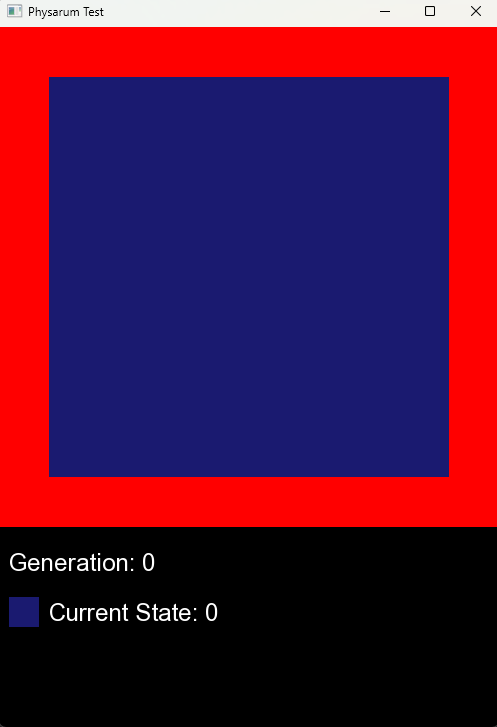
\includegraphics[width=0.5\textwidth]{./images/Pruebas/simulador/image001.png}
        \caption{Lienzo de 10 x 10}
        \label{fig:10x10}
    \end{figure}
    \vskip 0.5cm
    Posteriormente se colocaron los estados correspondientes a
    el estado inicial y al nutriente no encontrado.
    \vskip 0.5cm
    %FIgura
    \begin{figure}[htbp]
        \centering
        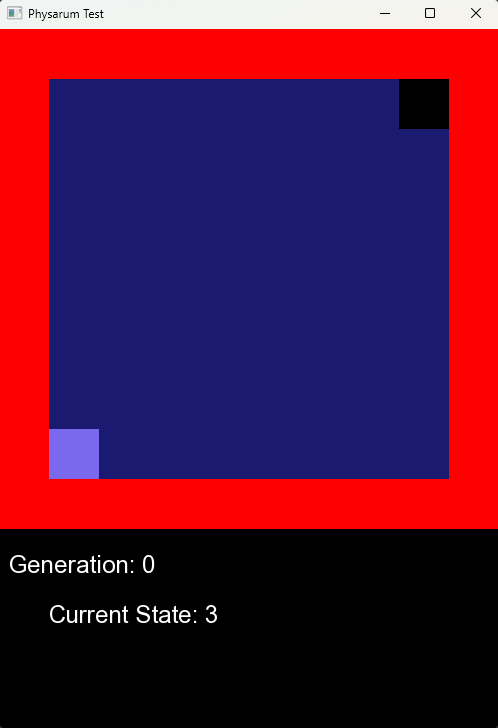
\includegraphics[width=0.5\textwidth]{./images/Pruebas/simulador/image002.png}
        \caption{Estados iniciales}
        \label{fig:Estados iniciales}
    \end{figure}
    \vskip 0.5cm
    Una vez colocada la configuraci\'on inicial, entonces se
        procede a iniciar la simulaci\'on, con la cual, al terminar las
        iteraciones se genera una ruta que va desde el estado inicial
        al nutriente no encontrado, el cual para este momento ha
        cambiado su estado a nutriente encontrado, cambiando a su
        vez el color correspondiente a este estado.
    \vskip 0.5cm
    %FIgura
    \begin{figure}[htbp]
        \centering
        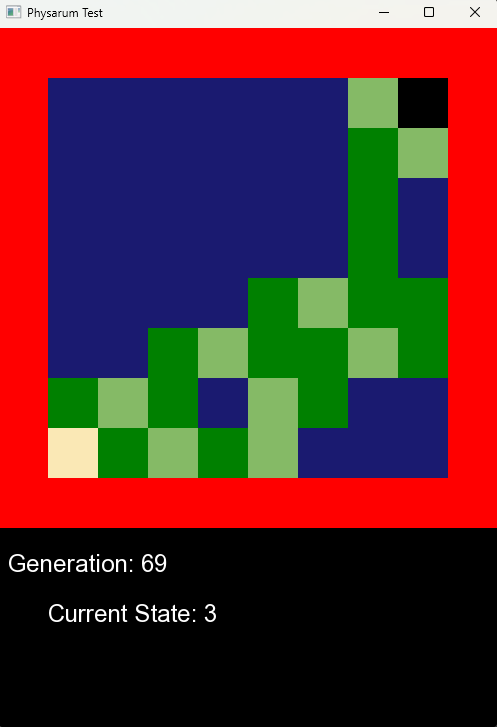
\includegraphics[width=0.5\textwidth]{./images/Pruebas/simulador/image003.png}
        \caption{Ruta encontrada}
        \label{fig:Ruta encontrada}
    \end{figure}
    \vskip 0.5cm
    En el programa es posible ver en qu\'e generaci\'on es en la que
        se encuentra el algoritmo, adem\'as del estado en el cual en ese
        momento se tiene elegido en el teclado, esto para ser
        colocado en el lienzo.
    \vskip 0.5cm
    Es posible colocar otra configuraci\'on una vez reiniciando el
        programa, donde se puede colocar los estados en distinta
        posici\'on, por lo que se muestran a continuaci\'on distintas
        configuraciones una vez finalizadas las simulaciones
        correspondientes a cada una de ellas.
    \vskip 0.5cm
    %FIgura
    \begin{figure}[htbp]
        \centering
        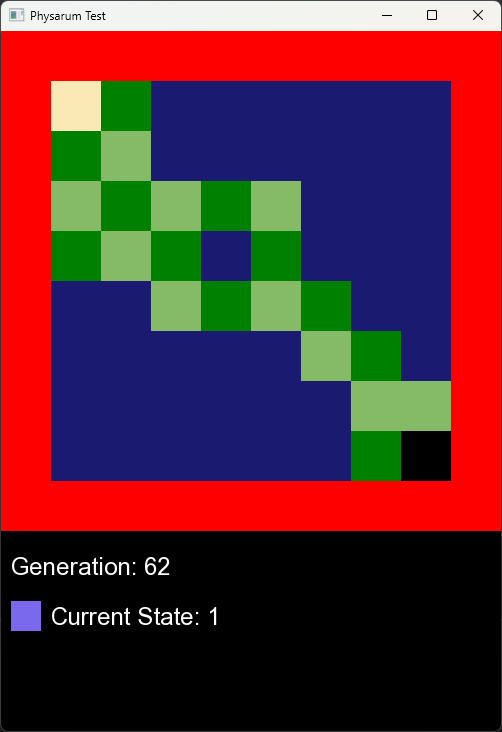
\includegraphics[width=0.5\textwidth]{./images/Pruebas/simulador/image004.png}
        \caption{Configuraci\'on 2}
        \label{fig:10x10}
    \end{figure}
    \vskip 0.5cm
    %FIgura
    \begin{figure}[htbp]
        \centering
        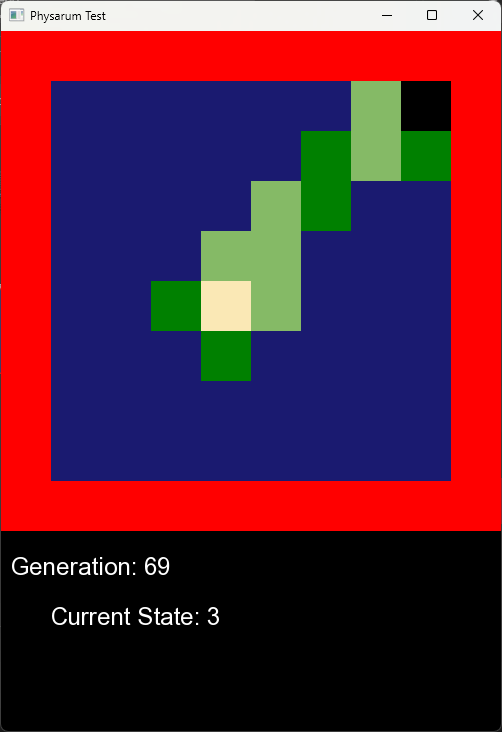
\includegraphics[width=0.5\textwidth]{./images/Pruebas/simulador/image005.png}
        \caption{Configuraci\'on 3}
        \label{fig:Estados iniciales}
    \end{figure}
    \vskip 0.5cm
    %FIgura
    \begin{figure}[htbp]
        \centering
        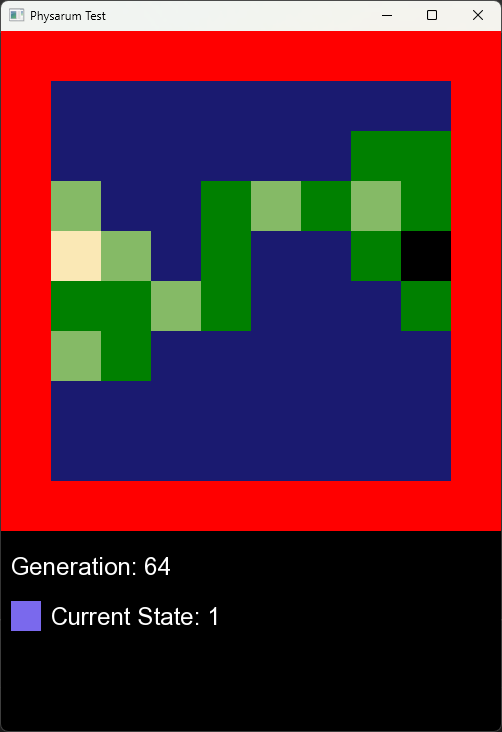
\includegraphics[width=0.5\textwidth]{./images/Pruebas/simulador/image006.png}
        \caption{Configuraci\'on 4}
        \label{fig:Ruta encontrada}
    \end{figure}
    \vskip 0.5cm
    Las simulaciones realizadas nos han devuelto resultados
        satisfactorios, debido a que las rutas son correctamente
        generadas de acuerdo a las reglas plasmadas en el algoritmo,
        yendo del punto inicial al final, y finalizando una vez que el
        Physarum ya no tiene la necesidad de expandirse, debido a
        que ha encontrado el nutriente que estaba buscando.
    \clearpage
% subsubsection subsubsection name (end)